\documentclass[10pt]{beamer}

%%%
% PREAMBLE FOR THIS DOC 
%%%
%https://tex.stackexchange.com/questions/68821/is-it-possible-to-create-a-latex-preamble-header
\usepackage{/Users/miw267/Repos/latex_preamble/beamer_preamble}


%%%
% DOCUMENT
%%%

\begin{document}

%\maketitle

%% Title page frame
%\begin{frame}
%    \titlepage 
%\end{frame}



\title{10/30/2026: Algorithm Efficiency}
\author{CSCI 246: Discrete Structures}
\date{Textbook reference: Sec 11.3, Epp}

\begin{frame}
    \titlepage 
\end{frame}


\begin{frame}
%\small
%\begin{mygreenbox}[title=Graded Quiz Pickup]
%Quizzes are in the front of the room, grouped into four bins (A-G, H-L, M-R, S-Z) by last name. The quizzes are upside down with your last name on the back. Come find yours before, during, or after class. Only turn the quiz over if it's yours.
%\end{mygreenbox} 
%\vfill 
\begin{myredbox}[title=Announcements]
\begin{itemize}
	\item The slides from Wednesday's class had two typos; they have been fixed.
\end{itemize}
\end{myredbox}

\vfill 
\begin{myyellowbox}[title=Today's Agenda]
\begin{itemize}
\item Quiz \#8 
\item Mini-lecture on algorithmic efficiency 
\item Group Exercises
\end{itemize}

\end{myyellowbox}
\vfill 

\end{frame}

\begin{frame}{Weekly Quiz \#8}

\begin{enumerate}
	\item \textit{(Induction.)}   Show by induction that $2^n < n!$ for all $n \geq 4$.	
	\item \textit{(Recurrence.)} Solve the Tower of Hanoi recursion: $a_n = 2 a_{n-1} + 1$ with $a_0=1$.
	\item \textit{(Recurrence.)} Show how to \enquote{outsmart} an intelligence test by finding a polynomial expression (of degree 3) for $a_n$ such that $a_0=1, a_1=2$, $a_2=4, a_3=8$, but $a_4=15$.
\end{enumerate}
\vfill 
\scriptsize 
\begin{mygreenbox}[title=\text{Reference Material: Solving first-order recurrences (Props 23.1, 23.3)}]
All solutions to recurrence relation $a_n = s a_{n-1} + t$ have the form
\[
a_n = 
\begin{cases}
c_1 s^n + c_2, & \text{ if } s \neq 1 \\
a_0 + nt, & \text{ if } s = 1 \\
\end{cases}
\]
\end{mygreenbox}

\begin{mygreenbox}[title=\text{Reference Material: Expressing a sequence with a polynomial (Thm 23.17)}]
Let $a_0, a_1, a_2, \hdots$ be a sequence of numbers. The terms $a_n$ can be expressed as polynomial expressions in $n$ if and only if there is a nonnegative integer $k$ such that for all $n \geq 0$ we have $\Delta^{k+1} a_n = 0$. In that case,
\[a_n = a_0 \binom{n}{0} +  (\Delta a_0) \binom{n}{1}  + (\Delta^2 a_0) \binom{n}{2} + \cdots + (\Delta^k a_0) \binom{n}{k}  \]
\end{mygreenbox}


\end{frame}




\begin{frame}[standout]
Mini-lecture
\end{frame}

\begin{frame}[fragile]
\small 
\begin{myredbox}[title=Practice Reading Quiz (Algorithm Efficiency)]
Assume $n$ is a positive integer and consider the following Python code:


\begin{python}
p=0; x=2
for i in range(2, n + 1):       # i = 2, 3, ..., n
	p=(p+i)*x
\end{python}


\begin{enumerate}
	\item What is the actual number of elementary operations that are performed when this algorithm segment is executed? Justify your answer.
	\item What is the order for this algorithm segment? Justify your answer.
\end{enumerate}
\end{myredbox}
\end{frame}



\begin{frame}[fragile]
\small
\begin{mygreenbox}[title=Solution to Practice Reading Quiz]

\begin{python}
p=0; x=2
for i in range(2, n + 1):       # i = 2, 3, ..., n
	p=(p+i)*x
\end{python}

\begin{enumerate}
	\item What is the actual number of elementary operations that are performed when this algorithm segment is executed?   \pause \alert{By the blue box below, $(n-1) \times 2 = 2n-2$.}  
	\item<4-> What is the order for this algorithm segment? \only<5->{\alert{By the theorem on polynomial orders, $\Theta(n)$.}}
\end{enumerate}
\end{mygreenbox}

\vfill
\only<2->{
\begin{mybluebox}[title=The number of elementary operations performed by a for loop]
The number of elementary operations performed by a for loop is given by
\[ \#  \text{elementary ops} \; = \; \#  \text{iterations}   \; \times \; \frac{\# \text{elementary ops}}{\text{iteration}} \]	
\end{mybluebox}
}

\end{frame}


\begin{frame}[fragile]{Nested for loops}
\footnotesize 
\colorbox{yellow!30}{\textbf{Poll.}} Consider an algorithm segment with a nested for loop, such as the one below.

\begin{myredbox}[title=\text{An algorithm segment with a nested for loop}]

\begin{python}
for i in range(1, n + 1):       # i = 1, 2, ..., n
    for j in range(1, i + 1):   # j = 1, 2, ..., i
        print("YOLO.")
\end{python}

\vspace{-.2cm}
\end{myredbox}
\vfill 
\pause 
How many times is the inner loop run?

\vfill 
\pause 

\colorbox{green!30}{\textbf{Solution.}}  The number of times the inner loop is run is 
\[1+2+3+4+ \hdots + n \]

\vfill 
\pause 
\colorbox{blue!30}{\textbf{Why do we care?}} We need this quantity to compute algorithmic efficiency:


\begin{mybluebox}[title=\text{The number of elementary operations performed by a \underline{nested} for loop}]
The number of elementary operations performed by a  \underline{nested} for loop is given by
\[ \#  \text{elementary ops} \; = \; \#  \text{ \underline{inner} iterations}   \; \times \; \frac{\# \text{elementary ops}}{\text{ \underline{inner} iteration}} \]	
\end{mybluebox}

\end{frame}



\begin{frame}

\begin{mygreenbox}[title=\text{Theorem: Sum of the first $n$ natural numbers}]
\small 
For every natural number $n \geq 1$, 
\[ 1 + 2 + \cdots + n = \frac{n \, (n+1)}{2} \]
\end{mygreenbox}
\vfill 
\pause 
\begin{myyellowbox}[title=\text{Story: Gauss' solution from elementary school}]
\begin{figure}
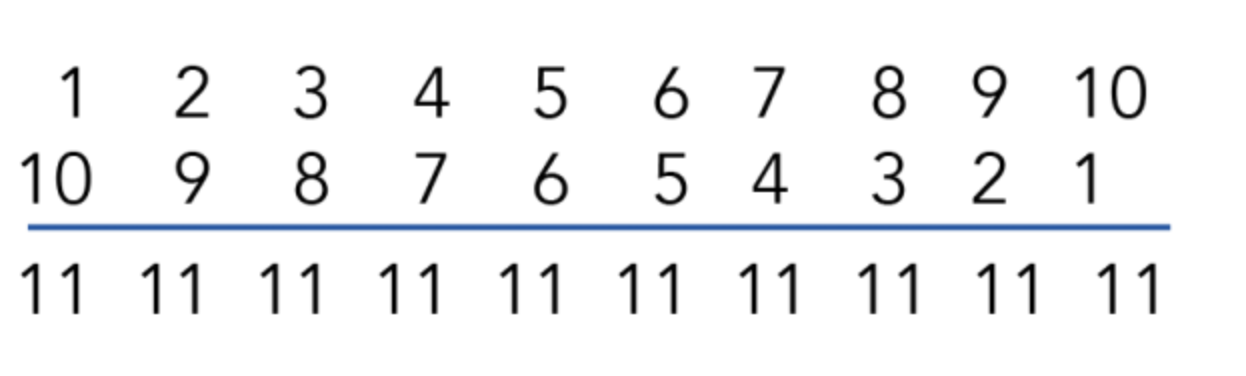
\includegraphics[width=\textwidth]{images/gauss_sum.png}	
\end{figure}	
\end{myyellowbox}
\vfill 
\pause 
\colorbox{red!30}{\textbf{Remark.}} Recall that we can use summation notation to express the left-hand side more succinctly; in that case, we write the theorem as:
\[ \sum_{k=1}^n k =  \frac{n \, (n+1)}{2} \]
\end{frame}


\begin{frame}[fragile]{Nested for loops}
\footnotesize 
\colorbox{yellow!30}{\textbf{Poll.}} 1. What is the number of elementary operations performed by the code block below? 2. What is the order for this algorithm segment? Justify your answer.

\begin{myredbox}[title=\text{An algorithm segment (in Python) with a nested for loop }]
\begin{python}
x=0
for i in range(1, n + 1):       # i = 1, 2, ..., n
    for j in range(1, i + 1):   # j = 1, 2, ..., i
        x=x+i*j
\end{python}
\vspace{-.2cm}
\end{myredbox}
\vfill 
\pause 


\begin{mybluebox}[title=\text{The number of elementary operations performed by a \underline{nested} for loop}]
The number of elementary operations performed by a  \underline{nested} for loop is given by
\[ \#  \text{elementary ops} \; = \; \#  \text{ \underline{inner} iterations}   \; \times \; \frac{\# \text{elementary ops}}{\text{ \underline{inner} iteration}} \]	
\end{mybluebox}

\vfill 
\pause 
\colorbox{yellow!30}{\textbf{Solution to \#1.}}
\only<3>{
\[ \alert{(1+ 2 + 3 + \hdots + n)} \cdot 2 \]
}
\only<4>{
\begin{align*}
\alert{(1+ 2 + 3 + \hdots + n)} \cdot 2 &= 	\alert{\frac{n(n+1)}{2}} \cdot 2 
\end{align*}
}

\only<5>{
\begin{align*}
\alert{(1+ 2 + 3 + \hdots + n)} \cdot 2 &= 	\alert{\frac{n(n+1)}{2}} \cdot 2 = n(n+1)
\end{align*}
}

\only<6->{
\begin{align*}
\alert{(1+ 2 + 3 + \hdots + n)} \cdot 2 &= 	\alert{\frac{n(n+1)}{2}} \cdot 2 = n(n+1) = n^2+n
\end{align*}
}

\only<7->{
\colorbox{yellow!30}{\textbf{Solution to \#2.}}
} \only<8->{ By the theorem on polynomial orders, $\Theta(n^2)$.}
\end{frame}




\begin{frame}{Remark: Big O is not \qq{worst case} complexity}

\begin{columns}[c]
    \column{0.4\textwidth}
    \centering
    \textbf{Method for computing} \\
    \textbf{\# elem. operations} \\
    Worst Case \\
   	Best Case  \\
	Average Case

    \column{0.1\textwidth}
    \centering
	{\Huge $\times$}
    
    \column{0.5\textwidth}
    \centering
    \textbf{Method for expressing} \\
    \textbf{order of algorithm} \\
    Big O \\
   	Big Theta  \\
	Big Omega

\end{columns}
	
\end{frame}

\begin{frame}{Big O is not \qq{worst case} complexity -- Example}

\begin{figure}
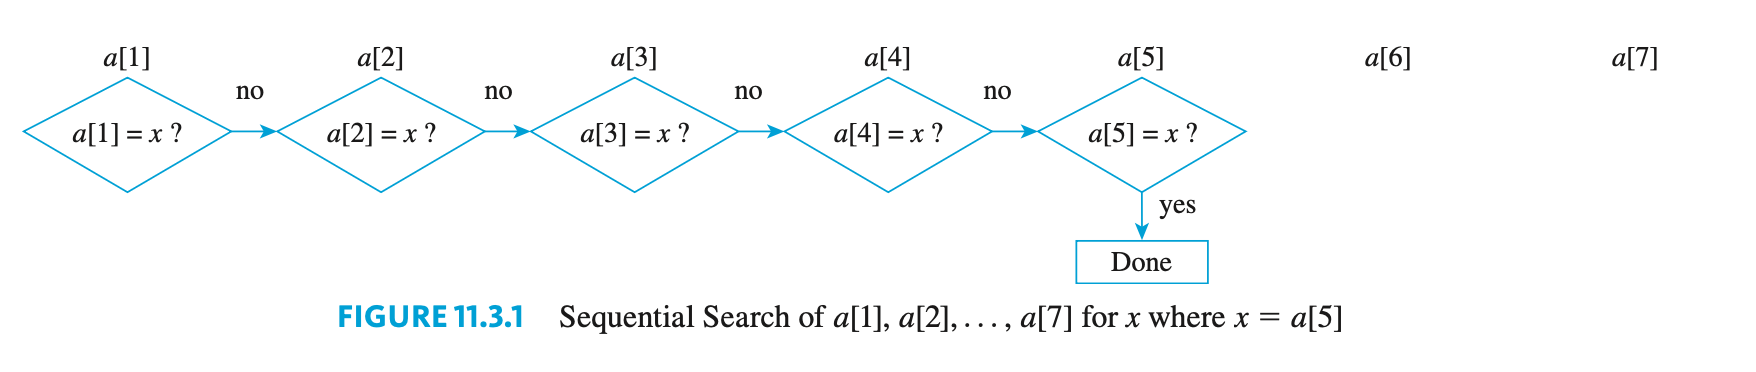
\includegraphics[width=\textwidth]{images/sequential_search.png}
\end{figure}

\vfill 
\pause 
\colorbox{yellow!30}{\textbf{Poll.}} How many elementary operations are required by sequential search over $n$ items in (a) the best case scenario, (b) the worst case scenario, (c) the average case scenario?

\vfill 
\pause 
\colorbox{green!30}{\textbf{Solution.}}  (a) 1 comparison \pause (b) $n$ comparisons \pause (c) $\frac{n+1}{2}$ comparisons (if the item of interest is equally likely to be anywhere in the array).

\vfill 
\pause 
\colorbox{blue!30}{\textbf{Remark.}} Hence, the order in each case is (a) $\Theta(1)$,   (b) $\Theta(n)$,  (c) $\Theta(n)$.  
\pause 
\vfill 
Thus, an upper bound on the order for each case is (a) $O(1)$,   (b) $O(n)$,  (c) $O(n)$. Likewise, a lower bound on the order for each case is (a) $\Omega(1)$,   (b) $\Omega(n)$,  (c) $\Omega(n)$.
	
\end{frame}


\begin{frame}{Two separate questions}
\colorbox{yellow!30}{\textbf{Question 1. Which inputs?}} \; Choosing a \textbf{case} gives a \textbf{function} of $n$:
\begin{itemize}
\item $W(n)$ = number of operations on the \textbf{worst} input of size $n$
\item $B(n)$ = number of operations on the \textbf{best} input of size $n$
\item $A(n)$ = \textbf{average} number of operations over inputs of size $n$
\end{itemize}
\vfill
\pause
\colorbox{green!30}{\textbf{Question 2. How do we describe that function?}}
\begin{itemize}
\item $O(g)$: grows \textbf{at most} like $g$ \quad (upper bound)
\item $\Omega(g)$: grows \textbf{at least} like $g$ \quad (lower bound)
\item $\Theta(g)$: grows \textbf{exactly} like $g$ \quad (both)
\end{itemize}
\vfill
\pause
\begin{mybluebox}[title=\text{Take-away}]
Cases (worst/best/average) pick \textit{which function} to study.  $O$, $\Omega$, $\Theta$ describe \textit{how fast it grows}.  Any case can be paired with any symbol.
\end{mybluebox}
\end{frame}

\begin{frame}{Example: sequential search over $n$ items}
\centering
\begin{tabular}{l c | c c c}
 & \textbf{\# comparisons} & $O$ & $\Omega$ & $\Theta$ \\
\hline
\textbf{Best case}    & $1$ & $O(1)$ & $\Omega(1)$ & $\Theta(1)$ \\
\textbf{Worst case}   & $n$ & $O(n)$ & $\Omega(n)$ & $\Theta(n)$ \\
\textbf{Average case} & $\frac{n+1}{2}$ & $O(n)$ & $\Omega(n)$ & $\Theta(n)$
\end{tabular}

\vfill
\pause
\raggedright
\colorbox{red!30}{\textbf{Note.}} All nine entries are true statements.  For example, ``the worst case is $\Omega(n)$'' is a perfectly good \textit{lower} bound on the \textit{worst} case.
\end{frame}

\begin{frame}{Big O is not \qq{worst case} complexity  -- Summary}

You’ll hear \qq{Big O means worst case.} It’s a common shorthand because people usually bound the worst case from above, but O is really an upper bound, and you can upper-bound any case. 
\vfill 
Theoretical computer scientists care just as much about lower bounds on the worst case, like $\Omega(n  \log n)$ for sorting.

	
\end{frame}


\begin{frame}[standout]
Group exercises
\end{frame}

\begin{frame}{Random group assignments}
\begin{columns}
\begin{column}{0.33\textwidth}
Ashley, Isabelle: 9 \\ 
Bailey, Tanna: 9 \\ 
Blaisdell, Olyver: 4 \\ 
Brown, Ashton: 1 \\ 
Cardenas, Dominic: 10 \\ 
Cutler, George: 1 \\ 
Fabik, Roland: 7 \\ 
Fellows, Audrey: 6 \\ 
Fitzgerald, Ryan: 6 \\ 
Fuller, Ryan: 3 \\ 
Griffen, Clara: 3 \\ 
Grutsch, Tanner: 5 \\\end{column}
\begin{column}{0.33\textwidth}
Hager, Nathan: 7 \\ 
Horner, Jayden: 8 \\ 
Johnson, Jaret: 2 \\ 
Kintzel, Samantha: 12 \\ 
Lameres, Alexis: 5 \\ 
Lee, Holden: 4 \\ 
Mayala, Reece: 10 \\ 
McLean, Connor: 2 \\ 
Mcbride, Daniel: 4 \\ 
Miller, Maverick: 7 \\ 
Moss, Emily: 10 \\ 
Mousseau, Matthew: 12 \\\end{column}
\begin{column}{0.33\textwidth}
Neuman, Evan: 11 \\ 
Putnam, John: 8 \\ 
Ramos, Vydel: 5 \\ 
Rathbun, Jedidiah: 11 \\ 
Roberts, Matthew: 6 \\ 
Roller, Nathan: 2 \\ 
Ryan, Otis: 1 \\ 
Shevtsov, Timothy: 11 \\ 
Stensland, Emma: 12 \\ 
Thiessen, Logan: 8 \\ 
Thompson, Jaiden: 3 \\ 
Vath, Ethan: 9 \\\end{column}
\end{columns}
\end{frame}

\begin{frame}[fragile]{Group exercises}
For each of the algorithm segments below, assume $n$ is a positive integer. 
\begin{itemize}
\item[a.] Compute the actual number of elementary operations (additions, subtractions, multiplications, divisions, and comparisons) that are performed when the algorithm segment is executed.  For simplicity, however, count only comparisons that occur within the body of the for loops; ignore those required to determine when the for loops should terminate. 
\item[b.] Use the theorem on polynomial orders to find an order for the algorithm segment.	
\end{itemize}



\centering
\begin{minipage}{0.32\textwidth}
% i = 3, 4, ..., n-1
    \centering
    \footnotesize Segment 1 \\
    \vspace{.2cm}
	\begin{python}[basicstyle=\ttfamily\scriptsize, numbers=none, columns=fullflexible, keepspaces=true]
for i in range(3, n):
    a = 3*n + 2*i - 1
	\end{python}
\end{minipage}
\hfill
\begin{minipage}{0.32\textwidth}
    \centering
    \small Segment 2 \\
      \vspace{.2cm}
	\begin{python}[basicstyle=\ttfamily\tiny, numbers=none, columns=fullflexible, keepspaces=true]
	for k in range(1,n):
		for j in range(1, k):
    		x = a[k] + b[j]
	\end{python}
\end{minipage}
\hfill
\begin{minipage}{0.32\textwidth}
    \centering
     \small Segment 3 \\
       \vspace{.2cm}
 	\begin{python}[basicstyle=\ttfamily\tiny, numbers=none, columns=fullflexible, keepspaces=true]
	for i in range(1,n+1):
		m = np.floor((i+1)/2)
		for j in range(1,m+1):
    		a=(n-i)*(n-j)
   	\end{python}
\end{minipage}
\end{frame}


\begin{frame}[fragile]{Solution for algorithm segment \#1}

\begin{python}[basicstyle=\ttfamily\normalsize, numbers=none]
for i in range(3, n):
    a = 3*n + 2*i - 1
\end{python}

\colorbox{green!30}{\textbf{Solution Summary.}}
\[ 
\begin{array}{lll}
\text{Step 1} & \textbf{\# its.} & n-3 \\
\text{Step 2} & \textbf{\# el ops. per it.} & 4 \\
\text{Step 3}& \textbf{\# el ops.} & 4n-12 \\
\text{Step 4} & \textbf{Order} & \Theta(n) \\
\end{array}
\]

\colorbox{red!30}{\textbf{Solution Details.}}
\[ 
\begin{array}{ll}
\text{Step 1} & \text{Since we skip the first two iterates, do $(n-1) - 2 = n-3$.} \\
\text{Step 2} & \text{Two multiplications, one subtraction, one addition.} \\
\text{Step 3}& \text{Multiply Steps 1 and 2.} \\
\text{Step 4} & \text{By theorem on polynomial orders.}\\
\end{array}
\]
    	
\end{frame}



\begin{frame}[fragile]{Solution for algorithm segment \#2}
\footnotesize 

	\begin{python}[basicstyle=\ttfamily\normalsize, numbers=none]
	for k in range(1,n):
		for j in range(1, k):
    		x = a[k] + b[j]
	\end{python}
\vfill 
\colorbox{green!30}{\textbf{Solution Summary.}}
\[ 
\begin{array}{lll}
\text{Step 1} & \textbf{\# its.} & \frac{n^2}{2} + \frac{n}{2}-1 \\
\text{Step 2} & \textbf{\# el ops. per it.} & 1 \\
\text{Step 3}& \textbf{\# el ops.} & \frac{n^2}{2} + \frac{n}{2}-1 \\
\text{Step 4} & \textbf{Order} & \Theta(n^2) \\
\end{array}
\]

\colorbox{red!30}{\textbf{Solution Details.}}
\[
\begin{array}{>{\RaggedRight\arraybackslash}p{1cm}>{\RaggedRight\arraybackslash}p{8cm}}
\text{Step 1} &  We unfold the nested loop into a single loop by focusing only on the inner loop. The inner loop does $2+ \hdots +n = \frac{n(n+1)}{2} -1$ iterations. Here we use Gauss' formula for summing the first $n$ natural numbers. \\
\text{Step 2} &  One addition. \\
\text{Step 3}& Multiply Steps 1 and 2. \\
\text{Step 4} & By theorem on polynomial orders. \\
\end{array}
\]
\end{frame}



\begin{frame}[fragile]{Solution for algorithm segment \#3}
\footnotesize 

\setlength{\columnsep}{0pt} % <--- This removes space between columns

\begin{columns}[c]
    % Left column: image
    \column{0.3\textwidth}
 	\begin{python}[basicstyle=\ttfamily\tiny, numbers=none, columns=fullflexible, keepspaces=true]
	for i in range(1,n+1):
		m = np.floor((i+1)/2)
		for j in range(1,m+1):
    		a=(n-i)*(n-j)
   	\end{python}
    % Right column: colored label + array
    \column{0.75\textwidth}
    \colorbox{green!30}{\textbf{Solution Summary.}} \\[0.3em]
    \[
    \begin{array}{lll}
    \text{Step 1} & \textbf{\# its.} & \begin{cases}
       \frac{n^2}{4} + \frac{n}{2}, & \text{$n$ even} \\
    \frac{n^2}{4} + \frac{n}{2} + \frac{1}{4}, & \text{$n$ odd} 
    \end{cases} \\
    \text{Step 2} & \textbf{\# el ops. per it.} & 3 \\
    \text{Step 3} & \textbf{\# el ops.} & \begin{cases}
        3\left(\frac{n^2}{4} + \frac{n}{2}\right), & \text{$n$ even}\\
    3\left(\frac{n^2}{4} + \frac{n}{2} + \frac{1}{4}\right), & \text{$n$ odd} 
    \end{cases} \\
    \text{Step 4} & \textbf{Order} & \Theta(n^2)
    \end{array}
    \]
\end{columns}


\colorbox{red!30}{\textbf{Solution Details.}}
How many times is the inner loop run? 
Depends if $n$ is odd or even.
 %
 \begin{align*}
 \texttt{\# its ($n$ even)} & = 1+1 + 2 +2 + \hdots + \frac{n}{2} + \frac{n}{2} \\
&= 2 \sum_{k=1}^{\frac{n}{2}} k  \stackrel{*}{=} \cancel{2} \frac{1}{\cancel{2}} (\frac{n}{2})(\frac{n+2}{2}) =    \frac{n^2}{4} + \frac{n}{2} \\
\texttt{\# its ($n$ odd)} & = 1+1 + 2 +2 + \hdots + \frac{n-1}{2} + \frac{n-1}{2} + \frac{n+1}{2} \\
&= 2 \sum_{k=1}^{\frac{n-1}{2}} k + \frac{n+1}{2} \stackrel{*}{=} \cancel{2} \frac{1}{\cancel{2}} (\frac{n-1}{2})(\frac{n+1}{2}) + \frac{n+1}{2} =  \frac{n^2}{4} + \frac{n}{2} + \frac{1}{4} 
 \end{align*}
%
In the equations marked *, we use Gauss' formula for summing the first $n$ natural numbers. 
\end{frame}

\end{document}
